% Options for packages loaded elsewhere
\PassOptionsToPackage{unicode}{hyperref}
\PassOptionsToPackage{hyphens}{url}
\PassOptionsToPackage{dvipsnames,svgnames,x11names}{xcolor}
%
\documentclass[
  11pt,
  letterpaper,
]{article}
\usepackage{amsmath,amssymb}
\usepackage{lmodern}
\usepackage{iftex}
\ifPDFTeX
  \usepackage[T1]{fontenc}
  \usepackage[utf8]{inputenc}
  \usepackage{textcomp} % provide euro and other symbols
\else % if luatex or xetex
  \usepackage{unicode-math}
  \defaultfontfeatures{Scale=MatchLowercase}
  \defaultfontfeatures[\rmfamily]{Ligatures=TeX,Scale=1}
\fi
% Use upquote if available, for straight quotes in verbatim environments
\IfFileExists{upquote.sty}{\usepackage{upquote}}{}
\IfFileExists{microtype.sty}{% use microtype if available
  \usepackage[]{microtype}
  \UseMicrotypeSet[protrusion]{basicmath} % disable protrusion for tt fonts
}{}
\makeatletter
\@ifundefined{KOMAClassName}{% if non-KOMA class
  \IfFileExists{parskip.sty}{%
    \usepackage{parskip}
  }{% else
    \setlength{\parindent}{0pt}
    \setlength{\parskip}{6pt plus 2pt minus 1pt}}
}{% if KOMA class
  \KOMAoptions{parskip=half}}
\makeatother
\usepackage{xcolor}
\IfFileExists{xurl.sty}{\usepackage{xurl}}{} % add URL line breaks if available
\IfFileExists{bookmark.sty}{\usepackage{bookmark}}{\usepackage{hyperref}}
\hypersetup{
  pdftitle={Parental loss from a global perspective},
  colorlinks=true,
  linkcolor={blue},
  filecolor={Maroon},
  citecolor={blue},
  urlcolor={blue},
  pdfcreator={LaTeX via pandoc}}
\urlstyle{same} % disable monospaced font for URLs
\usepackage[margin=25mm]{geometry}
\usepackage{longtable,booktabs,array}
\usepackage{calc} % for calculating minipage widths
% Correct order of tables after \paragraph or \subparagraph
\usepackage{etoolbox}
\makeatletter
\patchcmd\longtable{\par}{\if@noskipsec\mbox{}\fi\par}{}{}
\makeatother
% Allow footnotes in longtable head/foot
\usepackage{footnote} % For some unknown reason, footnotehyper clashes with French
\makesavenoteenv{longtable}
\usepackage{graphicx}
\makeatletter
\def\maxwidth{\ifdim\Gin@nat@width>\linewidth\linewidth\else\Gin@nat@width\fi}
\def\maxheight{\ifdim\Gin@nat@height>\textheight\textheight\else\Gin@nat@height\fi}
\makeatother
% Scale images if necessary, so that they will not overflow the page
% margins by default, and it is still possible to overwrite the defaults
% using explicit options in \includegraphics[width, height, ...]{}
\setkeys{Gin}{width=\maxwidth,height=\maxheight,keepaspectratio}
% Set default figure placement to htbp
\makeatletter
\def\fps@figure{htbp}
\makeatother
\setlength{\emergencystretch}{3em} % prevent overfull lines
\providecommand{\tightlist}{%
  \setlength{\itemsep}{0pt}\setlength{\parskip}{0pt}}
\setcounter{secnumdepth}{5}
\newlength{\cslhangindent}
\setlength{\cslhangindent}{1.5em}
\newlength{\csllabelwidth}
\setlength{\csllabelwidth}{3em}
\newlength{\cslentryspacingunit} % times entry-spacing
\setlength{\cslentryspacingunit}{\parskip}
\newenvironment{CSLReferences}[2] % #1 hanging-ident, #2 entry spacing
 {% dont indent paragraphs
  \setlength{\parindent}{0pt}
  % turn on hanging indent if param 1 is 1
  \ifodd #1
  \let\oldpar\par
  \def\par{\hangindent=\cslhangindent\oldpar}
  \fi
  % set entry spacing
  \setlength{\parskip}{#2\cslentryspacingunit}
 }%
 {}
\usepackage{calc}
\newcommand{\CSLBlock}[1]{#1\hfill\break}
\newcommand{\CSLLeftMargin}[1]{\parbox[t]{\csllabelwidth}{#1}}
\newcommand{\CSLRightInline}[1]{\parbox[t]{\linewidth - \csllabelwidth}{#1}\break}
\newcommand{\CSLIndent}[1]{\hspace{\cslhangindent}#1}

%%%%%%%% START HEADER PARTIAL %%%%%%%%%%%%

% Formatting of tables & knitr::kable and kableExtra functionality
\usepackage{float}
\usepackage{colortbl}
\usepackage{pdflscape}
\usepackage{tabu}
\usepackage{threeparttable}

% Line numbering

% endfloat stuff

% fancyhdr pagestyle

% Environment for keywords
\makeatletter
\newcommand\keywordsname{Keywords}
\newenvironment*{keywords}[1][\keywordsname]{\if@twocolumn \else \small \quotation \fi \begin{center} \textbf{\textit{#1} \\}}{\end{center}\if@twocolumn \else \small \endquotation \fi}
\newenvironment*{keywordsinline}[1][\keywordsname]{\if@twocolumn \else \small \quotation \fi \begin{center} \textbf{\textit{#1}: }}{\end{center}\if@twocolumn \else \small \endquotation \fi}
\makeatother

% Environment for abstract that takes new abstract name
\newenvironment{renameableabstract}[1][\abstractname]{\let\oldabstractname\abstractname \renewcommand{\abstractname}{#1} \begin{abstract}}{\end{abstract} \renewcommand{\abstractname}{\oldabstractname}}

%%%%%%%% END HEADER PARTIAL %%%%%%%%%%%%

\ifLuaTeX
  \usepackage{selnolig}  % disable illegal ligatures
\fi

\title{Parental loss from a global perspective}

%%%%%%% START AUTHOR PARTIAL %%%%%%%%%%%%%%%

%%%%% Authors, affiliations and author notes stuff %%%%%

% Macros for creating and referencing stored reference
\makeatletter
\def\MyNewLabel#1#2#3{\expandafter\gdef\csname #1@#2\endcsname{#3}}

\def\MyRef#1#2{\@ifundefined{#1@#2}{???}{\csname #1@#2\endcsname}}

\newcommand*\ifcounter[1]{%
  \ifcsname c@#1\endcsname
    \expandafter\@firstoftwo
  \else
    \expandafter\@secondoftwo
  \fi
}
\makeatother

% Create labels for Addresses if the are given by code
\MyNewLabel{ADDRTXT}{A}{Department of Statistical Sciences, University of Toronto, Canada}
\MyNewLabel{ADDRTXT}{B}{Leverhulme Centre for Demographic Science, University of Oxford, England}
\MyNewLabel{ADDRTXT}{C}{Max Planck Institute for Demographic Research, Germany}
\MyNewLabel{ADDRTXT}{D}{Departments of Statistical Sciences and Sociology, University of Toronto, Canada}

% Create labels for Footnotes if they are given by code
\MyNewLabel{ANOTETXT}{corresp}{\href{mailto:benjamin.schluter@utoronto.ca}{\nolinkurl{benjamin.schluter@utoronto.ca}}.}

%%% Special footnotes for addresses and author footnotes
\usepackage{bigfoot}
\DeclareNewFootnote{Addr}[arabic] % Only used for NOT authblk
\DeclareNewFootnote{ANote}[fnsymbol]

%%% Address and author notes as a function of format %%%
 % Use authblk for affiliations %%%%%%%%%%%
\usepackage{authblk}

% Always separate by commas
\renewcommand\Authsep{, }
\renewcommand\Authand{, }
\renewcommand\Authands{, }

% Counter for addresses and footnotes
\newcounter{addrcnt}

% thanks definition that doesnt produce superscript marks
\makeatletter
\newcommand*\createaddrlblbycode[1]{%
  \ifcounter{ADDRLBL@#1}
    {}
    {\refstepcounter{addrcnt}\newcounter{ADDRLBL@#1}\setcounter{ADDRLBL@#1}{\value{addrcnt}}}%
}

\newcommand*\addrlblbycode[1]{\arabic{ADDRLBL@#1}}

\newcommand*\addrbycode[1]{%
  \ifcounter{ADDR@#1}
    {}
    {\newcounter{ADDR@#1}%
     \affil[\addrlblbycode{#1}]{\MyRef{ADDRTXT}{#1}}}%
}

\newcommand*\createanotelblbycode[1]{%
  \ifcounter{ANOTELBL@#1}
    {}
    {\refstepcounter{footnoteANote}\newcounter{ANOTELBL@#1}\setcounter{ANOTELBL@#1}{\value{footnoteANote}}}%
}

\newcommand*\anotelblbycode[1]{\fnsymbol{ANOTELBL@#1}}

\newcommand*\anotebycode[1]{%
  \ifcounter{ANOTE@#1}
    {}
    {\newcounter{ANOTE@#1}%
     \footnotetextANote[\value{ANOTELBL@#1}]{\MyRef{ANOTETXT}{#1}}}%
}
\makeatother


\createaddrlblbycode{A}


\createanotelblbycode{corresp}

\author[%
\addrlblbycode{A}%
,%
$\anotelblbycode{corresp}$%
]{Benjamin-Samuel Schlüter}

\addrbycode{A}


\createaddrlblbycode{B}



\author[%
\addrlblbycode{B}%
]{Antonino Polizzi}

\addrbycode{B}


\createaddrlblbycode{C}



\author[%
\addrlblbycode{C}%
]{Diego Alburez-Gutierrez}

\addrbycode{C}


\createaddrlblbycode{D}



\author[%
\addrlblbycode{D}%
]{Monica Alexander}

\addrbycode{D}


%endif(authblk)

%%%%%%%%% END AUTHOR PARTIAL %%%%%%%%

\date{}

\begin{document}
\maketitle

%%%%%%%%%% START AFTER TITLE PARTIAL %%%%%%%%%%%%%
\anotebycode{corresp}


%%%%%%%%%% END AFTER TITLE PARTIAL %%%%%%%%%%%%%

\begin{abstract}
150 words
\end{abstract}

\hypertarget{introduction}{%
\section{Introduction}\label{introduction}}

\hypertarget{data-and-method}{%
\section{Data and Method}\label{data-and-method}}

Two sources of data were needed in order to estimate the worldwide parental loss by cause of death: cause-specific mortality, and life table data with its associated population counts, fertility rates and birth counts.

Period \emph{life table data} by 1-year age class (0, 1, 2, \ldots, 100+) and sex, grouped in one calendar year were obtained from the UN world population prospects (\protect\hyperlink{ref-united2022world}{United Nations 2022}). All the life table functions (e.g.~age-specific probabilities of dying and surviving) were retrieved from this data source. Yearly age-specific \emph{fertilty rates} for females aged 15 to 49 years old and \emph{population counts} by 1-year age group and sex were also obtained from this source.

\emph{Cause of death} information was obtained from modeled data from the Institute for Health Metrics and Evaluation (\protect\hyperlink{ref-ihme2019gbd}{2019}). Cause of death information was collected from this source for ages 0, 1-4, and then in five-year age groups until the open age-group 95 and more. We converted these counts into 1-year age group until age 100+, using a penalized composite link model (\protect\hyperlink{ref-rizzi2015efficient}{Rizzi, Gampe, and Eilers 2015}). Twenty-two causes of death were selected corresponding to the level two of the GBD hierarchy of causes.

We used the kinship matrix model (\protect\hyperlink{ref-caswell2019formal}{Caswell 2019}) where the projected kin was the parent (mother and father).\\
The model combined several extensions to use time-varying and sex-differentiated vital rates while accounting for death from multiple causes (\protect\hyperlink{ref-caswell2022formal}{Caswell 2022}; \protect\hyperlink{ref-caswell2023formal}{Caswell, Margolis, and Verdery 2023}; \protect\hyperlink{ref-caswell2021formal}{Caswell and Song 2021}). The parents' dynamics can be expressed as follows

\[\begin{pmatrix} \boldsymbol{d}^f_L \\ 
\boldsymbol{d}^m_L \\ 
\hline \boldsymbol{d}^f_D \\ 
\boldsymbol{d}^m_D 
\end{pmatrix}(x+1, t+1) = 
\left(\begin{array}{@{}c|c@{}}
  \begin{matrix} 
  \boldsymbol{U}^f_t & \boldsymbol{0} \\ 
  \boldsymbol{0} & \boldsymbol{U}^m_t 
  \end{matrix} & \boldsymbol{0} \\
\hline
\begin{matrix} 
  \boldsymbol{M}^f_t & \boldsymbol{0} \\ 
  \boldsymbol{0} & \boldsymbol{M}^m_t 
  \end{matrix} & \boldsymbol{0} \\
\end{array}\right)
\begin{pmatrix} \boldsymbol{d}^f_L \\ 
\boldsymbol{d}^m_L \\ 
\hline \boldsymbol{d}^f_D \\ 
\boldsymbol{d}^m_D
\end{pmatrix}(x, t)\]

where the matrix \(\boldsymbol{U}_t\) of dimension \((\omega \times \omega)\) contains the survival probabilities on its main subdiagonal; the matrix \(\boldsymbol{M}_t\) of dimension \((\alpha\omega \times \omega)\) contains the probabilities of dying from the causes considered on its main diagonals; \(\boldsymbol{d}_L\) refers to the age distribution of the parent living and \(\boldsymbol{d}_D\) reflects the age distribution of the parent dying by cause, in year \(t\) when a child is aged \(x\); upper scripts \(f\) and \(m\) corresponds to female and male, respectively; subscript \(t\) refers to the year; \(\omega=101\) which was the number of ages considered and \(\alpha=22\) as we considered twenty-two different causes of death. The block matrix on the right-hand side allows to project the parents' age distribution (alive or dead) over time, as their child ages. The model is fit on each country separately.\\
The model requires as input the age distribution of parents of offspring (see Caswell and Song (\protect\hyperlink{ref-caswell2021formal}{2021}) for more details). We assumed that in a given year \(t\), both parents were alive at the time of birth and the age distribution of parents at the birth of their child (when \(x=0\)) is expressed as \(\boldsymbol{\pi_t} = \frac{\boldsymbol{f}_t \circ \boldsymbol{n}_t}{||\boldsymbol{f}_t \circ \boldsymbol{n}_t||}\), where \(\boldsymbol{f}_t\) is a vector of dimension \((\omega \times 1)\) containing age-specific fertility rates and \(\boldsymbol{n}_t\) is a vector of dimension \((\omega \times 1)\) being the age distribution of the overall population. Hence, at the birth of a child in year \(t\),

\[\begin{pmatrix} \boldsymbol{d}^f_L \\ 
\boldsymbol{d}^m_L \\ 
\hline \boldsymbol{d}^f_D \\ 
\boldsymbol{d}^m_D 
\end{pmatrix}(0, t)
=
\begin{pmatrix} \boldsymbol{\pi_t}^f \\ 
\boldsymbol{\pi_t}^m \\ 
\hline \boldsymbol{0} \\ 
\boldsymbol{0} 
\end{pmatrix}
\]

We assumed that female and male age-specific fertility rates were equal as the UN does not provide male fertility.
Cause-specific mortality was not available for the period 1950-1990. During this period, we simplified the block-matrix to only contain survival probabilities, meaning that we only projected the age distribution of parents alive before 1990 (\(\boldsymbol{M}_t = \boldsymbol{0}\) for \(t < 1990\)). We additionally recorded the age distribution of parents dying by cause from 1990 onward. As it is commonly done in these models, before 1950, we assumed that the earliest available rates have been operating for a long time (stable population assumption).

Two metrics - obtained using outputs from the parents' dynamics - were of particular interest. First, the probability of bereavement of a randomly selected child in the population was approximated by

\[\text{Prob.(losing at least one parent)}(x,t)=1-(1-d_t/2)^2\]

where \(d_t\) represents the mean number of dead parent at age \(x\) of their child in year \(t\) (\protect\hyperlink{ref-caswell2023formal}{Caswell, Margolis, and Verdery 2023}).\\
Second, the percentage of born children aged less than 18 years old losing a parent in year \(t\) (\(PCLP_t\)). We computed it as follows

\[PCLP_t = \frac{\sum^{17}_{x=0}(l_{x,t} \cdot B_t) \cdot \text{Prob.(losing at least one parent)}(x,t)}{B_t}\]

where \(l_{x,t}\) corresponds to the fraction of the hypothetical cohort surviving to age \(x\) in the period life table for both sex combined in year \(t\) (using the same data as for \(\boldsymbol{U_t}\) but not differentiating by sex); and \(B_t\) is the number of births in year \(t\). This metric can also be made cause-specific by replacing \(\text{Prob.(losing at least one parent)}(x,t)\) by \(\text{Prob.(losing at least one parent due to cause i)}(x,t)\).

\hypertarget{preliminary-results}{%
\section{Preliminary Results}\label{preliminary-results}}

\begin{itemize}
\item
  Percentages always higher for father relative to mother (Fig. \ref{fig:perc-ber-all}).
\item
  Recent increase in Afghanistan driven by violent death (Fig. \ref{fig:perc-ber-all}-\ref{fig:perc-ber-top}).
\item
  HIV epidemics visible for Zimbabwe (Fig. \ref{fig:perc-ber-all}-\ref{fig:perc-ber-top}).
\end{itemize}

\begin{figure}
\centering
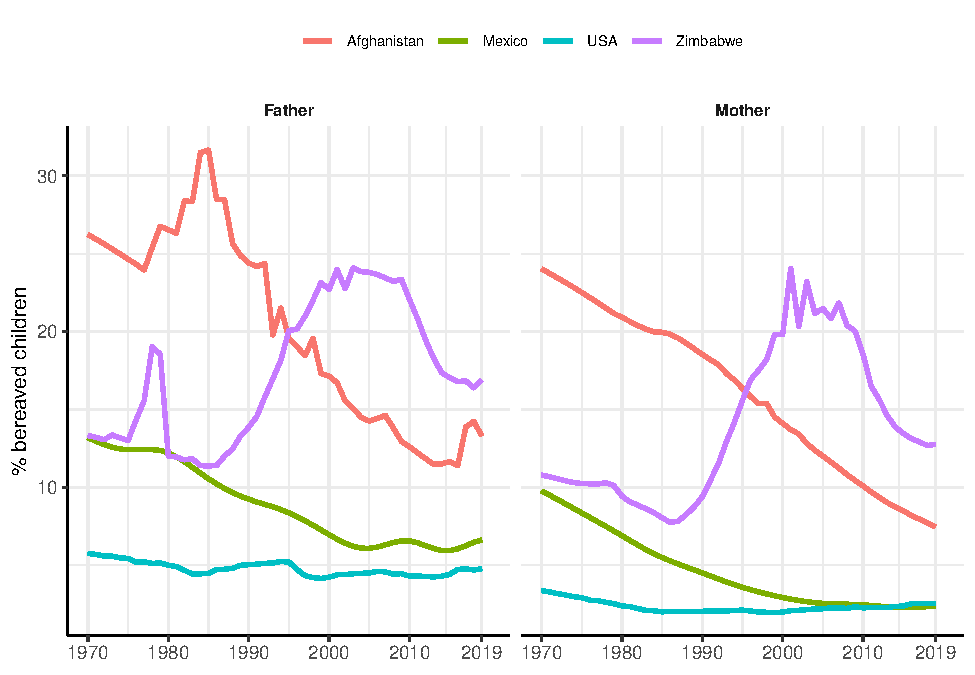
\includegraphics{parental_loss_global_paa_ext_abstract_files/figure-latex/perc-ber-all-1.pdf}
\caption{\label{fig:perc-ber-all}Percentage of children losing a parent, by parent sex and country over period 1970-2019}
\end{figure}

\begin{itemize}
\item
  Afghanistan and Mexico: top three parental causes of death vary between mother and father (Fig. \ref{fig:perc-ber-top}).
\item
  Global South: general downward trend except for father due to violent death in Mexico and Afghanistan, and HIV in Zimbabwe (Fig. \ref{fig:perc-ber-top}).
\end{itemize}

\begin{figure}
\centering
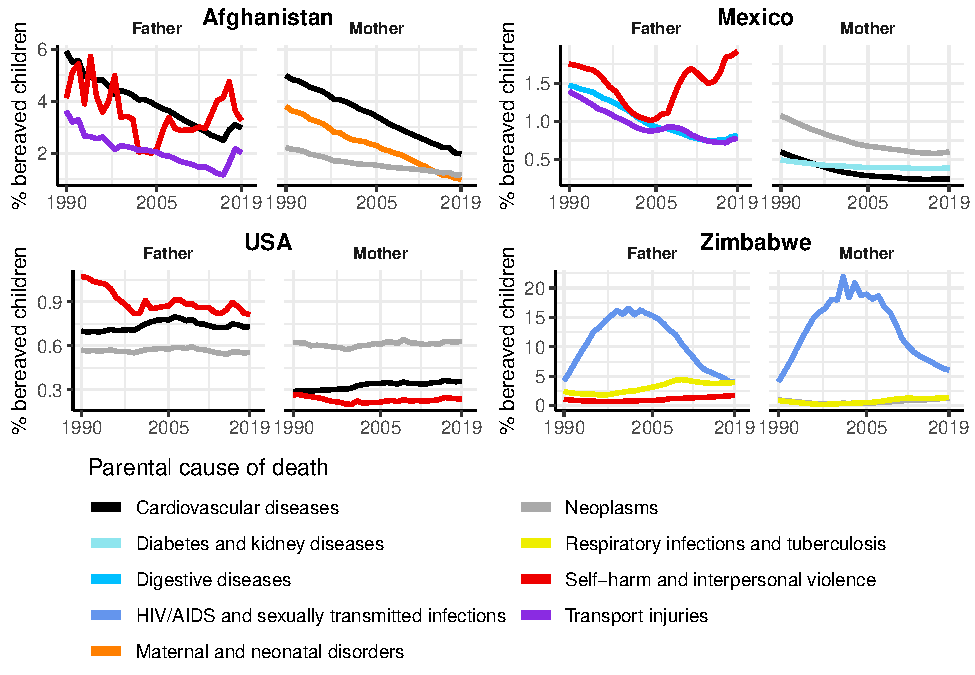
\includegraphics{parental_loss_global_paa_ext_abstract_files/figure-latex/perc-ber-top-1.pdf}
\caption{\label{fig:perc-ber-top}Percentage of children losing a parent, by parent sex and country top three causes of parental death over period 1990-2019}
\end{figure}

\begin{itemize}
\item
  Difference in the level of bereavement probability (Fig. \ref{fig:ber-prob}).
\item
  Difference in the mix of causes between the two countries (Fig. \ref{fig:ber-prob}).
\item
  Self-harm and transport injuries kill parents when their child are young (Fig. \ref{fig:ber-prob}).
\end{itemize}

\begin{figure}
\centering
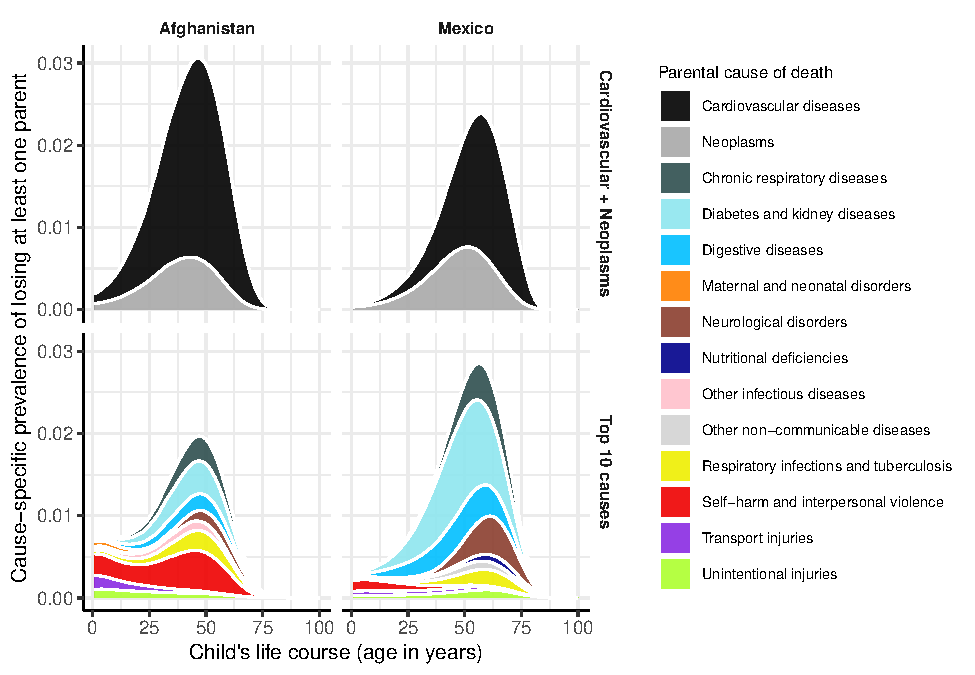
\includegraphics{parental_loss_global_paa_ext_abstract_files/figure-latex/ber-prob-1.pdf}
\caption{\label{fig:ber-prob}Age- and cause-specific bereavement probabilities of losing at least one parent, by country top twelve causes in 2019}
\end{figure}

\hypertarget{next-steps-extensions}{%
\section{Next Steps \& Extensions}\label{next-steps-extensions}}

\begin{itemize}
\item
  All countries
\item
  Uncertainty measures using posterior draws/95\% credible intervals
\item
  Validation with empirical data on US and Mexico
\item
  Projection using UN WPP projection estimates
\item
  Improve assumption about fertility of males
\end{itemize}

\newpage

\hypertarget{references}{%
\section*{References}\label{references}}
\addcontentsline{toc}{section}{References}

\hypertarget{refs}{}
\begin{CSLReferences}{1}{0}
\leavevmode\vadjust pre{\hypertarget{ref-caswell2019formal}{}}%
Caswell, H. (2019). The formal demography of kinship. \emph{Demographic Research} 41:679--712.

\leavevmode\vadjust pre{\hypertarget{ref-caswell2022formal}{}}%
Caswell, H. (2022). The formal demography of kinship IV. \emph{Demographic Research} 47:359--396.

\leavevmode\vadjust pre{\hypertarget{ref-caswell2023formal}{}}%
Caswell, H., Margolis, R., and Verdery, A.M. (2023). The formal demography of kinship v: Kin loss, bereavement, and causes of death. \emph{SocArXiv}. doi:\href{https://doi.org/10.31235/osf.io/mk64p}{10.31235/osf.io/mk64p}.

\leavevmode\vadjust pre{\hypertarget{ref-caswell2021formal}{}}%
Caswell, H. and Song, X. (2021). The formal demography of kinship III. \emph{Demographic Research} 45:517--546.

\leavevmode\vadjust pre{\hypertarget{ref-ihme2019gbd}{}}%
Institute for Health Metrics and Evaluation (2019). \emph{GBD Results}. University of Washington. \url{https://vizhub.healthdata.org/gbd-results/}.

\leavevmode\vadjust pre{\hypertarget{ref-rizzi2015efficient}{}}%
Rizzi, S., Gampe, J., and Eilers, P.H. (2015). Efficient estimation of smooth distributions from coarsely grouped data. \emph{American Journal of Epidemiology} 182(2):138--147.

\leavevmode\vadjust pre{\hypertarget{ref-united2022world}{}}%
United Nations (2022). \emph{World Population Prospects 2022: Summary of Results}. UN.

\end{CSLReferences}


\end{document}
